\chapter{Grundlagen} % (fold)
\label{sec:grundlagen}
Die folgenden Abschnitte sollen die theoretischen Grundlagen vermitteln, die notwendig sind, um das Thema dieser Thesis zu betrachten. Die Konzepte, die hier beschrieben werden sind relationale Algebra, Graphentheorie, APIs, als auch relationale und Graph Datenbanken.
\section{Relationale Algebra} % (fold)
\label{sec:relationaleAlgebra}
Die relationale Algebra ist ein mathematisches System, welches 1970 von E.F. Codd entwickelt wurde. Sie wird unter anderem zu Abfrage und Mutation von Daten in relationalen Datenbanken verwendet wird. Durch sie wird eine Menge an Operationen beschrieben, die auf die Relationen angewendet werden können, um neue Relationen zu bilden. \citep{relationalModel}

\subsection{Basisrelation} % fold
\label{sec:basisrelation}
Die Anwendung relationaler Algebra erfordert die Verwendung von Basisrelationen als fundamentale Bausteine, um mittels Grundoperationen komplexe Ausdrücke zu konstruieren, welche neue Relationen definieren. Eine Basisrelation setzt sich aus drei Komponenten zusammen: Tupel, Attributen und Domänen. Tupel reflektieren die Zeilen einer Tabelle, welche die einzelnen Datensätze repräsentieren. Diese werden durch Attribute in spezifische Spalten eingeteilt, welche die Eigenschaften der Tupel beschreiben. Die Wertebereiche, die für die einzelnen Attribute zulässig sind, werden als Domänen bezeichnet. Demnach ist jede Relation eine Menge von Tupeln mit spezifischen Attributen und deren Domänen. \citep{rdb}
%subsection basisrelation (end)

\subsection{Grundoperationen} % fold
\label{sec:grundoperationen}
Grundoperationen in der relationalen Algebra sind einfache mengentheoretische Operationen, die auf die Basisrelationen angewandt werden. Insgesamt gibt es sechs Grundoperationen, die nachfolgend erläutert werden.
\begin{itemize}
\item Bei der \textbf{Selektion $\sigma$} werden die einzelnen Tupel basieren auf einer Bedingung gefiltert. Ein Beispiel hierfür wäre  \colorbox{gray!20}{$\sigma$ Alter > 30 (Person)}. Hierdurch werden nur Personen mit einem Alter von mehr als 30 Jahren zurückgeliefert.
\item Die \textbf{Projektion $\pi$} ermöglicht es bestimmte Attribute einer Relation auszuwählen oder zu entfernen. Beispielsweise kann durch \colorbox{gray!20}{$\pi$ Name, Alter (Person)}, nur der Name und das Alter einer Person zurückgegeben werden.
\item Das \textbf{Kartesisches Produkt $\times$} kombiniert jede Zeile der ersten Relation mit jeder Zeile der zweiten Relation. Somit erzeugt  \colorbox{gray!20}{$R \times S$} alle möglichen Kombinationen aus \colorbox{gray!20}{R} und \colorbox{gray!20}{S}.
\item Eine \textbf{Vereinigung $\cup$} verknüpft die Tupel zweier Relationen, die eine gleiche Struktur aufweisen.  \colorbox{gray!20}{$R \cup S$} kombiniert somit alle Tupel aus beiden Relationen mit gleicher Struktur, ohne Duplikate zu erzeugen.
\item Die \textbf{Differenz  $\setminus$} zweier Relationen liefert alle Tupel, die in der ersten Relation vorkommen, aber nicht in der Zweiten. Sinngemäß gibt \colorbox{gray!20}{$R \setminus S$} alle Tupel \colorbox{gray!20}{R} aus die nicht in \colorbox{gray!20}{S} enthalten sind.
\item Der \textbf{Schnitt $\cap$} findet die Tupel, die in beiden Relationen vorhanden sind. Somit gibt \colorbox{gray!20}{$R \cap S$} die Tupel, die sowohl in \colorbox{gray!20}{R} als auch in \colorbox{gray!20}{S} entahlten sind zurück.
\end{itemize}
\noindent Durch die Verbindung dieser Grundoperationen können andere Operationen, wie beispielhaft ein Theat-Join $\bowtie$, welcher durch eine Kombination aus kartesischem Produkt und Selektion alle Tupel zweier Relationenen aufgrund einer Bedingung miteinander verbindet, erstellt werden.  \citep{rdb}
%subsection grundoperationen (end)
% section relationaleAlgebra (end)

\section{Graphentheorie} % (fold)
\label{sec:graphentheorie}
Ein Graph besteht im allgemeinen aus Knoten und verbindenden Kanten (vgl. Abb 1). In der Informatik bietet diese Datenstruktur einen großen Vorteil gegenüber der relationalen Algebra, wenn es sich um stark verzweigte Daten handelt. \citep{graphTheory}

\begin{figure}[h!]
	\centering
	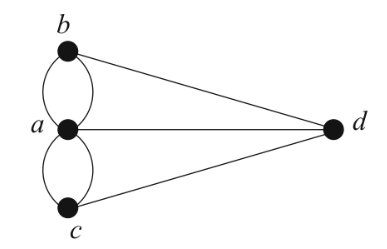
\includegraphics[scale=1]{Illustrations/graph.png}
	\caption{Modell eines ungerichteten Graphen. \citep{graphTheory}}
\end{figure}
\newpage
\subsection{Knoten} % fold
\label{sec:knoten}
Knoten sind Punkte innerhalb eines Graphen, die beispielsweise als Objekte der realen Welt verstanden werden können. Diese Objekte können zum Beispiel geographische Koordinaten sein, um einen Distanz-Graphen zu erstellen oder auch Webseiten, um einen Web-Graphen zu erhalten, der die Verbindung verschiedener Webseiten aufzeigt.
Innerhalb der Knoten unterscheidet man verschiedene Typen. Zum einen gibt es Isolierte Knoten. Diese besitzen keine Verbindung zu anderen Knoten des Graphens und können zur Identifizierung nicht-verbundener Teile eines Netzwerks verwendet werden. Außerdem gibt es verbundene Knoten, welche mindestens eine Verbindung zu einem andern Knoten besitzen. Dadurch ergibt sich eine dirkete Verbindung zu einem benachbarten Knoten. Außerdem kann eine Indirekte Verbindung enstehen, indem ein Pfad zwischen Ausgangs und Endknoten existiert, der über mehrere Verbindungen führt. \citep{graphTheory} \citep{graphapplication}
%subsection knoten (end)

\subsection{Kanten} % fold
\label{sec:kanten}
Kanten dienen in einem Graphen dazu, die Knoten miteinander zu Verbinden, um eine Relation zwischen ihnen zu visualisieren. Jede Kante besitzt einen Start- und Endknoten, der auch derselbe Knoten sein kann. Somit würde man in diesem Fall von einer Schleife sprechen. So wie es verschiedene Arten von Knoten gibt, exestieren auch verschiedene Kanten. 
In Abb. 2.1 sind \textit{ungerichtete Kanten} im Graphen zu sehen. Sie verbinden die Knoten auf die trivialste Art, indem sie ohne Richtung, Gewicht oder andere Beschränkung eine Verbindung herstellen. Durch ungerichtete Kanten ensteht ein ungerichteter Graph.
\textit{Gerichtete Kanten} werden in Abb. 2.2 (a) genutzt. Diese werden durch einen Pfeil visualisiert. Dieser gibt an, in welcher Richtung der Graph eine Beziehung zwischen den Knoten herstellt. Es ist ebenfalls möglich, dass zwei Knoten eine beidseitige Beziehung durch zwei gerichtete Kanten, also eine Kante pro Richtung, eingehen. Ein Graph, der durch gerichtete Kanten verbunden ist wird gerichteter Graph genannt.
Werden Zahlenwerte zu einer Kante hinzugefügt (vgl. Abb 2 (b)), so spricht man von \textit{gewichteten Kanten}. Diese können verwendet werden, um die Strecke zwischen zwei Kanten darzustellen oder die Kosten für die Nutzung der Kante anzugeben. Wird ein Graph mit gewichteten Kanten verbunden, spricht man von einem gewichteten Graphen.\citep{graphTheory} \citep{graphapplication}
\begin{figure}[H]
	\centering
	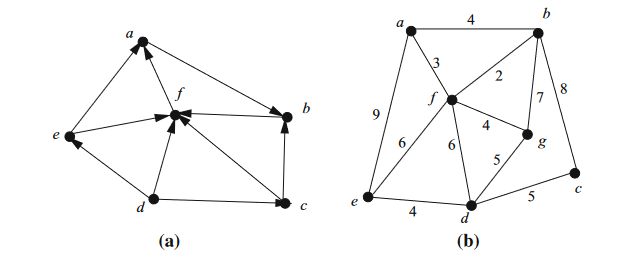
\includegraphics[scale=1]{Illustrations/graph_01.png}
	\caption{Modell eines gerichteten (a) und eines gewichtet Graphen (b). \citep{graphTheory}}
\end{figure}
%subsection kanten (end)

\subsection{Traversierung} % fold
\label{sec:traversierung}
Die Bewegung von einem Knoten oder einer Kante zu einem anderen in einem Graphen nach vorgegebenen Kriterien wird als Traversierung bezeichnet. Graphdatenbanken bieten in der Regel Traversalmechanismen, um Daten von miteinander verbundenen Knoten effizient abzufragen und abzurufen. \cite{graph}
%subsection traversierung (end)


% section graphentheorie (end)

\section{API} % (fold)
\label{sec:apigrundlagen}
Nachfolgend werden die Grundlagen von APIs thematisiert. Hierbei werden die grundlegenden Definitionen sowie die Typen vorgestellt, die für diese Arbeit von Relevanz sind.
\subsection{Definition API} % (fold)
\label{sec:grundlegendedefinitionvonapi}
Der Begriff \glqq API\grqq{}  steht für \glqq Application Programming Interface\grqq{}. Eine API bezeichnet eine Schnittstelle, welche Entwicklern den Zugriff auf Daten und Informationen ermöglicht. Bekannte Beispiele für häufig genutzte APIs sind die Twitter- und Facebook-APIs. Diese sind für Entwickler zugänglich und ermöglichen die Interaktion mit der Software von Twitter und Facebook. Zudem ermöglichen APIs die Kommunikation zwischen Anwendungen. Sie bieten den Anwendungen einen Weg, miteinander über das Netzwerk, überwiegend das Internet, in einer gemeinsamen Sprache zu kommunizieren. \citep{apistrategyguide}
%subsection grundlegendedefinitionvonapi (end)
\newpage
\subsection{REST API} % (fold)
\label{sec:restapi}
 \textbf{Representational State Transfer (REST)} wurde erstmals im Jahr 2000 in einer Dissertation von Roy Fielding beschrieben. Hierbei handelt es sich um einen Software-Architekturstil für APIs. REST basiert auf einer Ressourcenorientierung, bei der jede Entität als Ressource betrachtet und durch eine eindeutige Uniform Resource Locator (URL) identifiziert wird. Die Architektur basiert auf sechs grundlegenden Beschränkungen, darunter die Client-Server-Architektur, bei der Client und Server unabhängig voneinander agieren. Ein wesentlicher Bestandteil von REST ist die Zustandslosigkeit, d. h. jede Anfrage beinhaltet sämtliche für die Verarbeitung erforderlichen Informationen, wodurch die Interaktion zwischen Client und Server vereinfacht wird. Die Umsetzung der CRUD-Operationen (Create, Read, Update, Delete) erfolgt durch die HTTP-Methoden (POST, GET, PUT, DELETE). REST nutzt das in HTTP integrierte Caching, um die Antwortzeiten und die Leistung zu optimieren. Dabei besteht die Möglichkeit, Serverantworten als cachefähig oder nicht cachefähig zu kennzeichnen. Des Weiteren ist eine einheitliche Schnittstelle zu nennen, welche die Interaktionen zwischen unterschiedlichen Geräten und Anwendungen erleichtert. Darüber hinaus erfordert REST ein mehrschichtiges System, bei dem jede Komponente lediglich mit der unmittelbar vorgelagerten Schicht interagiert. RESTful APIs, die diesen Prinzipien folgen, nutzen HTTP-Anfragen, um Ressourcen effizient zu bearbeiten. \citep{Fielding2000}  \citep{graphqlreplacerest}

%subsection restapi (end) 
\subsection{GraphQL} % (fold)
\label{sec:graphql}
\textbf{GraphQL} wurde 2012 von Facebook für den internen Gebrauch entwickelt und 2015 als Open-Source-Projekt veröffentlicht. Das Kernkonzept von GraphQL basiert auf clientgetriebenen Abfragen, bei denen der Client die Struktur der Daten präzise definiert und nur die tatsächlich benötigten Daten anfordert. Diese clientseitige Steuerung reduziert die Menge der übertragenen Daten und führt zu effizienteren Netzwerkaufrufen, da nur die relevanten Informationen übermittelt werden. 
Im Vergleich zu REST verursacht GraphQL signifikant weniger Overhead, was die Netzwerkperformance optimiert. Die hierarchische Struktur der Abfragen, die die Graph-Struktur widerspiegelt, ermöglicht eine intuitive und flexible Datenmodellierung. Die starke Typisierung in GraphQL wird durch ein Schema definiert, das die Typen der Daten spezifiziert. Dies sorgt für eine verbesserte Validierung der Abfragen und bietet eine klarere Dokumentation. Im Gegensatz zu REST, bei dem für verschiedene Operationen mehrere Endpunkte erforderlich sind, nutzt GraphQL nur einen einzigen Endpunkt für alle API-Abfragen, was die Komplexität auf der Serverseite reduziert und eine vereinfachte API-Verwaltung ermöglicht. \citep{graphqlreplacerest}
%subsection graphql (end)
% section apigrundlagen (end)

\section{Datenbank} % (fold)
\label{sec:datenbankGrundlagen}
Im Folgenden werden die Grundlagen von Datenbanken behandelt. Es werden grundlegende Definitionen im Zusammenhang mit Datenbanken und die verschiedenen Arten von Datenbanken vorgestellt.
\subsection{Definition Datenbank und Datenbank Management System} % (fold)
\label{sec:definitiondatenbank}
Eine Datenbank stellt eine Sammlung von Daten und Informationen dar, welche für einen einfachen Zugriff gespeichert und organisiert werden. Dies umfasst sowohl die Verwaltung als auch die Aktualisierung der Daten. Die in der Datenbank gespeicherten Daten können nach Bedarf hinzugefügt, gelöscht oder geändert werden. Die Funktionsweise von Datenbanksystemen basiert auf der Abfrage von Informationen oder Daten, woraufhin entsprechende Anwendungen ausgeführt werden. DBMS bezeichnet eine Systemsoftware, die für die Erstellung und Verwaltung von Datenbanken eingesetzt wird. Zu den Funktionalitäten zählen die Erstellung von Berichten, die Kontrolle von Lese- und Schreibvorgängen sowie die Durchführung einer Nutzungsanalyse. Das DBMS fungiert als Schnittstelle zwischen den Endnutzern und der Datenbank, um die Organisation und Manipulation von Daten zu erleichtern. Die Kernfunktionen des DBMS umfassen die Verwaltung von Daten, des Datenbankschemas, welches die logische Struktur der Datenbank definiert, sowie der Datenbank-Engine, welche das Abrufen, Aktualisieren und Sperren von Daten ermöglicht. Diese drei wesentlichen Elemente dienen der Bereitstellung standardisierter Verwaltungsverfahren, der Gleichzeitigkeit, der Wiederherstellung, der Sicherheit und der Datenintegrität. \citep{9677042}

%subsubsection definitiondatenbank (end)

\subsection{Relationale Datenbank} % (fold)
\label{sec:relationaleDatenbanken}
Relationale Datenbanken basieren auf dem relationalen Modell, das von E.F. Codd entwickelt wurde und relationaler Algebra sowie Tuple-Relational-Kalkül zugrunde liegt. Sie speichern Daten in einer hochstrukturierten Tabellenform, wobei jede Tabelle aus Zeilen, den sogenannten Tupeln, und Spalten, den sogenannten Attributen, besteht. Jede Zeile repräsentiert einen Datensatz, während jede Spalte durch einen spezifischen Datentyp definiert ist. Die Struktur ermöglicht eine klare Organisation der Daten und erleichtert deren Verwaltung. Relationale Datenbanken verwenden Primär- und Fremdschlüssel, um Beziehungen zwischen Tabellen herzustellen und referenzielle Integrität zu gewährleisten, wodurch die Datenkonsistenz erhalten bleibt. Aufgrund dieser Eigenschaften werden die Tabellen häufig auch als "Relationen" bezeichnet. 

\newpage \noindent
Die bekanntesten RDBMS sind Microsoft SQL Server, Oracle MySQL und IBM DB2. Ein RDBMS organisiert alle Daten in tabellarischer Form und bietet Funktionen wie Primärschlüssel zur eindeutigen Identifikation von Datensätzen sowie Indizes, die die Geschwindigkeit der Datenabfragen erhöhen. Darüber hinaus unterstützen RDBMS die Erstellung virtueller Tabellen, die komplexe Abfragen vereinfachen, sowie einen kontrollierten Mehrbenutzerzugriff mit individueller Rechtevergabe. Die Verwendung einer standardisierten Sprache SQL ermöglicht die Verwaltung, Abfrage und Manipulation von Daten. Die genannten Merkmale machen relationale Datenbanken äußerst flexibel und benutzerfreundlich. 
Ein großer Vorteil relationaler Datenbanken liegt in ihrer Unterstützung der ACID-Prinzipien (Atomicity, Consistency, Isolation, Durability). Diese gewährleisten Stabilität und Sicherheit bei Transaktionen, was sie für viele Anwendungsbereiche geeignet macht. Darüber hinaus bieten sie eine hohe Datenintegrität, reduzieren Redundanz und ermöglichen die einfache Implementierung von Sicherheitsmaßnahmen.  Trotz dieser Vorteile stoßen relationale Datenbanken bei bestimmten Anforderungen an ihre Grenzen. Sie sind oft nicht für hohe Skalierbarkeit geeignet und können mit dem exponentiellen Wachstum von Daten schwer umgehen. Die Einrichtung und Wartung solcher Systeme ist häufig kostspielig, und die Verwaltung unstrukturierter Daten wie Multimedia oder Social-Media-Inhalte stellt eine große Herausforderung dar. Zudem erschwert die tabellarische Struktur komplexe Datenverknüpfungen und die Integration mehrerer Datenbanken.
Aufgrund dieser Einschränkungen haben moderne Anwendungen und Big-Data-Anforderungen zur Entwicklung von NoSQL-Datenbanken geführt, die besser auf die Verwaltung unstrukturierter und verteilter Daten ausgelegt sind. Dennoch bleiben relationale Datenbanken aufgrund ihrer Standardisierung, Benutzerfreundlichkeit und breiten Einsatzmöglichkeiten ein wesentlicher Bestandteil der Datenbanktechnologie.  \citep{relationalDatabase}  \citep{9677042}
%subsection relationaleDatenbanken (end)
\subsection{Graphdatenbanken} % (fold)
\label{sec:graphDatenbanken}
Graphdatenbanken sind spezialisierte Datenbanksysteme, die das Datenmodell dem User in Form eines Graphen präsentieren. Darüber hinaus enthalten die Graphen Informationen über die Eigenschaften der Knoten und Kanten, wodurch eine flexible und schemafreie Speicherung semistrukturierter Daten ermöglicht wird. Abfragen in Graphdatenbanken werden häufig als Traversalen formuliert, was ihnen gegenüber relationalen Datenbanken erhebliche Geschwindigkeitsvorteile verschafft, insbesondere bei komplexen Beziehungsabfragen.
Man unterscheidet zwischen nativen und nicht-nativen Graphdatenbanken. Native Graphdatenbanken sind speziell für das Graphmodell entwickelt und speichern die Daten intern in Graphenform. Nicht-native Graphdatenbanken hingegen verwenden andere Speichertechnologien, wie beispielsweise relationale Datenbanken, und präsentieren die Daten lediglich in Form von Graphen, um CRUD-Zugriffe zu ermöglichen. Beide Typen gehören zur Kategorie der NoSQL-Datenbanken, die durch den Verzicht auf das starre Tabellenschema relationaler Datenbanken deren Schwächen umgehen.
Durch ihre besondere Architektur bieten Graphdatenbanken nicht nur eine effiziente Verarbeitung von Beziehungsdaten, sondern erfüllen auch ACID-Bedingungen und unterstützen Rollbacks, was die Konsistenz der gespeicherten Informationen gewährleistet. Damit stellen sie eine leistungsstarke Alternative zu traditionellen relationalen Datenbanken dar, insbesondere in Anwendungsbereichen mit hochgradig verknüpften Daten.
\citep{9677042} \citep{graphdb} 
%subsection graphDatenbanken (end)
% section datenbankGrundlagen (end)

% chapter grundlagen (end)